\documentclass{report}
\usepackage[letterpaper,portrait,margin=2cm]{geometry}
\usepackage{titlesec}
\usepackage{amsmath,amssymb,amsthm}
\usepackage{tabularx}
\usepackage{enumitem}
\usepackage{indentfirst}
\usepackage{dsfont}
\usepackage{tikz}
\usepackage{hyperref}
\usepackage{mathtools}
\usepackage{mathrsfs}
\usepackage{enumitem}

\hypersetup{
	colorlinks=false
}

\renewcommand{\contentsname}{Table des mati\`eres}

\title{MAT346 - Analyse II

Donn\'e par Mario Lambert}
\author{Julien Houle}
\date{Automne 2025}

\NewDocumentCommand{\bornee}{O{a,b}}{\mathcal{B}\left[ #1 \right]}
\NewDocumentCommand{\continue}{O{a,b}}{\mathcal{C}\left[ #1 \right]}
\NewDocumentCommand{\riemann}{O{a,b}}{\mathcal{R}\left[ #1 \right]}
\NewDocumentCommand{\partitions}{O{a,b}}{\Omega\left[ #1 \right]}
\NewDocumentCommand{\msup}{mO{[a,b]}}{\overline{M}(#1,#2)}
\NewDocumentCommand{\minf}{mO{[a,b]}}{\underline{M}(#1,#2)}
\NewDocumentCommand{\ssup}{mO{\Delta}}{\overline{S}(#1,#2)}
\NewDocumentCommand{\sinf}{mO{\Delta}}{\underline{S}(#1,#2)}

\newcommand*{\Ssup}[1]{\overline{S}(#1)}
\newcommand*{\Sinf}[1]{\underline{S}(#1)}

\newcommand*{\raffinement}[2]{#1 \vee #2}
\newcommand*{\norme}[1]{\left\| #1 \right\|}
\newcommand*{\abs}[1]{\left| #1 \right|}

\newcommand*{\eps}{\varepsilon}

\newcommand*{\reels}{\mathbb{R}}
\newcommand*{\entiers}{\mathbb{Z}}
\newcommand*{\rationels}{\mathbb{Q}}
\newcommand*{\naturels}{\mathbb{N}}


\titleformat{\chapter}[hang]{\bfseries\huge\centering}{Chapitre \arabic{chapter}}{1em}{}[]
\titleformat{\section}[hang]{\bfseries\large}{Section \arabic{chapter}.\arabic{section}}{1em}{}[]
\titleformat{\subsection}[hang]{\bfseries\normalsize}{}{0pt}{}[]
\titleformat{\subsubsection}[hang]{\slshape\normalsize}{}{0pt}{}[]

\newtheorem*{thm}{Th\'eor\`eme}
\newtheorem*{lem}{Lemme}
\newtheorem*{prop}{Proposition}
\newtheorem*{coro}{Corollaire}
\theoremstyle{definition}
\newtheorem*{defin}{D\'efinition}
\theoremstyle{remark}
\newtheorem*{exem}{Exemple}
\newtheorem*{exer}{Exercice}
\newtheorem*{nota}{Notation}
\newtheorem*{rema}{Remarque}
\newtheorem*{rapp}{Rappel}

\begin{document}
	\maketitle
	\tableofcontents
	\newpage

	\chapter{Int\'egration}
	\section{Int\'egrales de Riemann}

	\begin{nota}
		~

		$\bornee[c,d]=\left\lbrace f:[a,b] \to \reels \middle| f \text{ est born\'ee} \right\rbrace$.

		$\riemann=\left\lbrace f:[a,b] \to \reels \middle| f \text{ est born\'ee et int\'egrable} \right\rbrace$.

		$\continue=\left\lbrace f:[a,b] \to \reels \middle| f \text{ est born\'ee et continue} \right\rbrace$.
	\end{nota}

	On suppose nos fonctions born\'ees.

	\begin{defin}
		~

		\begin{enumerate}[label=\alph*)]
			\item Une partition de $[a,b]$ est un ensemble fini de points $\Delta=\{x_0,x_1,\dotsc,x_n\} \subseteq [a,b]$ t.q. $a=x_0 < x_1 < x_2 < \dotsc < x_{n-1} < x_n=b$.
			\item L'ensemble des partitions de $[a,b]$ est $\partitions$.
			\item On dit $\Delta'$ est \emph{plus fine} que $\Delta$, not\'e $\Delta' \geq \Delta$, si $\Delta' \supseteq \Delta$.
			\item \emph{Raffinement commun} de $\Delta_1$ et $\Delta_2$, not\'e $\raffinement{\Delta_1}{\Delta_2}$, est la partition de $[a,b]$ form\'ee de $\Delta_1 \cup \Delta_2$ ordonn\'es.
			\item La \emph{norme} de $\Delta$, not\'ee $\norme{\Delta}$, est $\norme{\Delta}=\displaystyle\max\limits_{i=1}^{n}\abs{x_i-x_{i-1}}$.
			\item
			\begin{align*}
				\msup{f}[\left[ x_{i-1},x_1 \right]]&= \displaystyle\sup\limits_{x \in \left[ x_{i-1},x_1 \right]}f(x)\\
				\minf{f}[\left[ x_{i-1},x_1 \right]]&= \displaystyle\inf\limits_{x \in \left[ x_{i-1},x_1 \right]}f(x)
			\end{align*}
		\end{enumerate}
		\begin{rema}
			\begin{align*}
				\norme{x}&\geq0\\
				\norme{\lambda x}&=\abs{\lambda} \norme{x}\\
				\norme{x+y}&= \norme{x} + \norme{y}
			\end{align*}
		\end{rema}
	\end{defin}

	\begin{defin}
		~

		\begin{enumerate}[label=\alph*)]
			\item La \emph{somme de Riemann par exc\`es} (ou sup\'erieure) de $f$ pour la partition $\Delta$ est
			\[
			\ssup{f}= \displaystyle\sum_{i=1}^{n}\msup{f}[\left[ x_{i-1},x_i \right]] \cdot (x_i-x_{i-1})
			\]
			\item La \emph{somme de Riemann par d\'efaut} (ou inf\'erieure) de $f$ pour la partition $\Delta$ est
			\[
			\sinf{f}= \displaystyle\sum_{i=1}^{n}\minf{f}[\left[ x_{i-1},x_i \right]] \cdot (x_i-x_{i-1})
			\]
		\end{enumerate}
	\end{defin}

	\newpage
	\begin{prop}
		~

		\begin{enumerate}[label=\alph*)]
			\item
			\[
			\minf{f} \cdot (b-a) \leq \sinf{f}, \forall\Delta\in\partitions
			\]
			\item
			\[
			\sinf{f} \leq \ssup{f}
			\]
			\item
			\[
			\ssup{f} \leq \msup{f} \cdot (b-a)
			\]
		\end{enumerate}
	\end{prop}

	\begin{prop}
		Si $\Delta'\geq\Delta$, alors $\ssup{f}[\Delta']\leq\ssup{f}$.
		\begin{proof}[d\'emonstration]~

			Sans perte de g\'en\'eralit\'e, supposons
			\[
			\Delta:a=x_0<x_1<\dotsc<x_{i-1}<x_i<\dotsc<x_n=b
			\]
			\[
			\Delta':a=x_0<x_1<\dotsc<x_{i-1}<\bar{x}<x_i<\dotsc<x_n=b
			\]

			On a
			\begin{align*}
				\ssup{f}-\ssup{f}[\Delta']&= \left[ \msup{f}[\left[ x_{i-1},x_i \right]] \cdot (x_1-x_{i-1}) \right]\\
				&- \left[ \msup{f}[\left[ x_{i-1},\bar{x} \right]] \cdot (\bar{x}-x_{i-1}) + \msup{f}[\left[ \bar{x},x_i \right]] \cdot (x_i-\bar{x}) \right]\\
				&= (x_i-\bar{x}) \left[ \msup{f}[\left[ x_{i-1},x_i \right]] - \msup{f}[\left[ \bar{x},x_i \right]] \right]\\
				&+ (\bar{x}-x_{i-1}) \left[ \msup{f}[\left[ x_{i-1},x_i \right]] - \msup{f}[\left[ x_{i-1},\bar{x} \right]] \right]\\
				&\geq 0
			\end{align*}
		\end{proof}
	\end{prop}

	\begin{prop}
		Si $\Delta'\geq\Delta$, alors $\sinf{f}[\Delta'] \geq \sinf{f}$
		\begin{proof}[d\'emonstration]~

			\begin{center}
				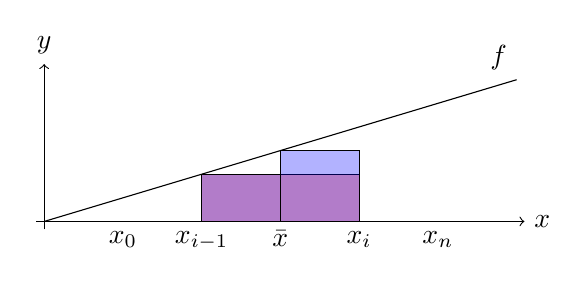
\begin{tikzpicture}
					\draw[->] (0,-.1) -- (0,2) node[above] {$y$};
					\draw[->] (-.1,0) -- (6.1,0) node[right] {$x$};
					\node[anchor=north] (x0) at (1,0) {$x_0$};
					\node[anchor=north] (xi-1) at (2,0) {$x_{i-1}$};
					\node[anchor=north] (x) at (3,0) {$\bar{x}$};
					\node[anchor=north] (xi) at (4,0) {$x_i$};
					\node[anchor=north] (xn) at (5,0) {$x_n$};
					\draw plot[domain=0:6] (\x,.3*\x) node[above left] {$f$};
					\node (y0) at (1,.3) {};
					\node (yi-1) at (2,.6) {};
					\node (y) at (3,.9) {};
					\node (yi) at (4,1.2) {};
					\node (yn) at (5,1.5) {};
					\filldraw[fill=red, fill opacity=.3] (yi-1) rectangle (xi.north);
					\filldraw[fill=blue, fill opacity=.3] (yi-1) rectangle (x.north);
					\filldraw[fill=blue, fill opacity=.3] (y) rectangle (xi.north);
				\end{tikzpicture}
			\end{center}
		\end{proof}
		\begin{rema}
			$\sinf{f}=-\ssup{-f}$.
		\end{rema}
		\begin{coro}
			$\forall \Delta_1,\Delta_2 \in \partitions, \sinf{f}[\Delta_1] \leq \ssup{f}[\Delta_2]$
			\begin{proof}[d\'emonstration]~

				On a $\raffinement{\Delta_1}{\Delta_2} \geq \Delta_1$. Ainsi,
				\begin{align*}
					\sinf{f}[\Delta_1]&\leq \sinf{f}[\raffinement{\Delta_1}{\Delta_2}]\\
					&\leq \ssup{f}[\raffinement{\Delta_1}{\Delta_2}]\\
					&\leq \ssup{f}[\Delta_2]
				\end{align*}
			\end{proof}
		\end{coro}
	\end{prop}

	\newpage
	\begin{defin}
		~

		\begin{enumerate}[label=\alph*)]
			\item La somme par d\'efaut de $f$ est $\Sinf{f}=\displaystyle\sup\limits_{\Delta\in\partitions}\sinf{f}$.
			\item La somme par exc\`es de $f$ est $\Ssup{f}=\displaystyle\inf\limits_{\Delta\in\partitions}\ssup{f}$.
		\end{enumerate}
	\end{defin}

	\begin{thm}
		$\Sinf{f} \leq \Ssup{f}$
		\begin{proof}[d\'emonstration]~

			Soit $\Delta_1 \in \partitions$

			$\Sinf{f}=\sup\sinf{f}$ est le plus petit majorant des $\sinf{f}$ avec $\Delta \in \partitions$.

			Du corollaire pr\'ec\'edant, on a que $\sinf{f} \leq \ssup{f}[\Delta_1]$.

			Donc, $\ssup{f}[\Delta_1]$ est un majorant des $\sinf{f}$.

			Ainsi, $\Sinf{f} \leq \ssup{f}[\Delta_1]$.

			De m\^eme, $\Ssup{f}=\inf\ssup{f}$ est le plus grand minorant des $\ssup{f}$ avec $\Delta \in \partitions$.

			Comme $\Sinf{f}$ est un minorant des $\ssup{f}$, on a que $\Sinf{f} \leq \Ssup{f}$.
		\end{proof}
	\end{thm}

	\begin{defin}
		~

		Soit $f \in \bornee$. On dit que $f$ est \emph{int\'egrable au sens de Riemann sur $[a,b]$} si $\Sinf{f}=\Ssup{f}$ et on note $f \in \riemann$. La valeur commune de $\Sinf{f}$ et $\Ssup{f}$ est not\'ee $\int_{a}^{b}f(x)\ dx$
	\end{defin}

	\addcontentsline{toc}{subsection}{Crit\`ere d'int\'egrabilit\'e}
	\begin{thm}[Crit\`ere d'int\'egrabilit\'e]
		~

		Soit $f \in \bornee$. Alors $f \in \riemann$ si, et seulement si, $\left( \forall \eps >0 \right) \left( \exists\Delta = \Delta(\eps) \in \partitions \right)$ t.q. $\ssup{f}-\sinf{f} < \eps$.
		\begin{proof}[d\'emonstration]~

			\begin{itemize}
				\item[$(\Rightarrow)$] Supposons $f \in \riemann$.

				Soit $\eps>0$.

				On a $\displaystyle\int_{a}^{b}f=\Ssup{f}=\inf\ssup{f}$.

				Comme $\Ssup{f}+\dfrac{\eps}{2}$ ne peut minorer $\ssup{f}$, alors $\exists\Delta_1 \in \partitions$ t.q. $\ssup{f}[\Delta_1] < \Ssup{f}+\dfrac{\eps}{2}$.

				De m\^eme, $\displaystyle\int_{a}^{b}f=\Sinf{f}=\sup\sinf{f}$.

				Comme $\Sinf{f}-\dfrac{\eps}{2}$ ne peut majorer $\sinf{f}$, alors $\exists\Delta_2 \in \partitions$ t.q. $\sinf{f}[\Delta_2] > \Sinf{f}-\dfrac{\eps}{2}$.

				Posons $\Delta = \Delta(\eps) = \raffinement{\Delta_1}{\Delta_2}$.

				On a
				\begin{align*}
					\ssup{f} - \sinf{f}&\leq \ssup{f}[\Delta_1] - \sinf{f}[\Delta_2]\\
					&< \Ssup{f} + \dfrac{\eps}{2} - \left( \Sinf{f} - \dfrac{\eps}{2} \right)\\
					&= \left( \Ssup{f} - \Sinf{f} \right) + \eps\\
					&= \eps
				\end{align*}
				\newpage
				\item[$(\Leftarrow)$] Soit $\eps>0$.

				Alors $\exists\Delta$ t.q. $\ssup{f}-\sinf{f}<\eps$.

				Mais alors,
				\begin{align*}
					\eps&> \ssup{f}-\sinf{f}\\
					&\geq \Ssup{f}-\Sinf{f}\\
					&\geq 0
				\end{align*}

				Du th\'eor\`eme du sandwich, $\Ssup{f}=\Sinf{f}$, car $\eps>0$ est arbitraire.

				Donc, $f \in \riemann$.
			\end{itemize}
		\end{proof}
		\begin{coro}
			S'il existe $\Delta \in \partitions$ t.q. $\ssup{f}=\sinf{f}$, alors $f \in \riemann$.
		\end{coro}
	\end{thm}
	\begin{thm}
		Toute fonction continue sur $[a,b]$ est int\'egrable sur $[a,b]$.
		\begin{proof}[d\'emonstration]~

			Soit $f \in \continue$.

			Soit $\eps>0$.

			Par la proposition d'Archim\`ede, $\exists n\in\entiers$ t.q. $n\eps>b-a$.

			\begin{rapp}~

				$f$ est uniform\'ement continue sur $[a,b]$ si $\left( \forall\eps>0 \right) \left( \exists\delta>0 \right)$ t.q. pour $x,y \in [a,b]$, $\abs{x-y}<\delta \Rightarrow \abs{f(x)-f(y)}<\eps$.
			\end{rapp}
			\begin{rapp}~

				Si $f$ est continue sur $[a,b]$, alors $f$ est uniform\'ement continue sur $[a,b]$.
			\end{rapp}

			Comme $f \in \continue$, elle est uniform\'ement continue sur $[a,b]$.

			Alors, $\exists\delta>0$ t.q. pour $x,y \in [a,b]$, $\abs{x-y}<\delta \Rightarrow \abs{f(x)-f(y)}<\frac{1}{n}$.

			Soit donc $\Delta \in \partitions: a=x_0<x_1,\dotsc<x_n=b$ avec $\norme{\Delta}<\delta$.

			Alors, $\msup{f}[\left[ x_{i-1},x_i \right]] - \minf{f}[\left[ x_{i-1},x_i \right]]<\frac{1}{n}$.
			\begin{rema}
				$\msup{f}[\left[ x_{i-1},x_i \right]] - \minf{f}[\left[ x_{i-1},x_i \right]]$ peut \^etre not\'e $\mathrm{osc}_f(\left[ x_{i-1},x_i \right])$.
			\end{rema}

			On obtient
			\begin{align*}
				\ssup{f}-\sinf{f}&= \sum_{i=1}^{n}\left[ \msup{f}[\left[ x_{i-1},x_i \right]] - \minf{f}[\left[ x_{i-1},x_i \right]] \right] \left( x_i-x_{i-1} \right)\\
				&< \dfrac{1}{n} \sum_{i=1}^{n}\left( x_i-x_{i-1} \right)\\
				&=\dfrac{b-a}{n}\\
				&< \eps
			\end{align*}

			Donc $f \in \riemann$.
		\end{proof}
	\end{thm}
	\begin{thm}
		Toute $f:[a,b] \to \reels$ monotone est int\'egrable.
		\begin{proof}[d\'emonstration]~

			\begin{enumerate}[label=(\arabic*)]
				\item Si $f$ est constante, alors $\ssup{f}-\sinf{f}=0<\eps$.
				\item Si $f$ est croissante,

				Soit $\eps>0$

				Soit $n \in \naturels$ t.q. $n\eps>(b-a)(f(b)-f(a))$

				Soit $\Delta:a=x_0<x_1<\dotsc<x_n=b$ avec $x_i=a+i\frac{b-a}{n}, i\in[0..n]$

				On a
				\begin{align*}
					\ssup{f}-\sinf{f}&= \sum_{i=1}^{n}\left[ \msup{f}[\left[ x_{i-1},x_i \right]] - \minf{f}[\left[ x_{i-1},x_i \right]] \right] (x_i-x_{i-1})\\
					&= \sum_{i=1}^{n}\left[ f(x_i) - f(x_{i-1}) \right] \left( \frac{b-a}{n} \right)\\
					&= \frac{b-a}{n} \left[ f(b)-f(a) \right]\\
					&< \eps
				\end{align*}

				Donc, $f \in \riemann$.
				\item Si $f$ est d\'ecroissante, alors $-f$ est croissante et $-f \in \riemann$.

				Donc, $f \in \riemann$.
			\end{enumerate}
		\end{proof}
	\end{thm}
	\begin{thm}
		~

		Si $f_1,f_2 \in \riemann$, alors $f_1+f_2 \in \riemann$ et $\int \left( f_1+f_2 \right) =\int f_1 + \int f_2$.
		\begin{proof}[d\'emonstration]~

			Soit $\eps>0$.

			Comme $f_i \in \riemann$, $\exists\Delta_i \in \partitions$ t.q. $\ssup{f_i}[\Delta_i]-\sinf{f_i}[\Delta_i]<\frac{\eps}{2}$.

			Soit $\Delta = \raffinement{\Delta_1}{\Delta_2}$.

			Alors, $\ssup{f_i}-\sinf{f_i}<\frac{\eps}{2}$.

			Supposons $\Delta:a=x_0<x_1<\dotsc<x_n=b$.

			On a
			\begin{align*}
				\ssup{f_1+f_2}&\leq \ssup{f_1} + \ssup{f_2}\\
				\sinf{f_1+f_2}&\geq \sinf{f_1} + \sinf{f_2}
			\end{align*}

			Car $\sup(f_1+f_2) \leq \sup f_1 + \sup f_2$ et $\inf(f_1+f_2) \geq \inf f_1 + \inf f_2$.

			Alors,
			\begin{align*}
				\ssup{f_1+f_2}-\sinf{f_1+f_2}&\leq \ssup{f_1} + \ssup{f_2} - \sinf{f_1} - \sinf{f_2}\\
				&< \frac{\eps}{2} + \frac{\eps}{2}\\
				&= \eps
			\end{align*}

			Donc, $f_1+f_2 \in \riemann$.

			De plus,
			\begin{align*}
				\int_{a}^{b}f_1+f_2&\leq \ssup{f_1+f_2}\\
				&\leq \ssup{f_1} + \ssup{f_2}\\
				&< \sinf{f_1}+\frac{\eps}{2} + \sinf{f_2}+\frac{\eps}{2}\\
				&\leq \int_{a}^{b}f_1+\frac{\eps}{2} + \int_{a}^{b}f_2+\frac{\eps}{2}
			\end{align*}

			Ainsi, $\int_{a}^{b}f_1+f_2 < \int_{a}^{b}f_1 + \int_{a}^{b}f_2 + \eps$, $\forall\eps>0$.

			Donc, $\int_{a}^{b}f_1+f_2 \leq \int_{a}^{b}f_1 + \int_{a}^{b}f_2$.

			De m\^eme, on peut montrer que $\int_{a}^{b}f_1+f_2 \geq \int_{a}^{b}f_1 + \int_{a}^{b}f_2$.

			Donc, $\int_{a}^{b}f_1+f_2 = \int_{a}^{b}f_1 + \int_{a}^{b}f_2$.
		\end{proof}
	\end{thm}
	\begin{thm}
		~

		Si $f \in \riemann$ et $\lambda \in \reels$, alors $\lambda f \in \riemann$ et $\int \lambda f = \lambda \int f$.
		\begin{proof}[d\'emonstration]~

			Laiss\'e en exercice.

			Utiliser $\frac{\eps}{\lambda}$ et $\ssup{\lambda f} = \lambda\ssup{f}$.
		\end{proof}
		\begin{coro}
			~

			Si $f,g \in \riemann$, alors $f \leq g \Rightarrow \int f \leq \int g$.
			\begin{proof}[d\'emonstration]~

				$g-f \geq 0 \Rightarrow \int g-f \geq 0 \Rightarrow \int g - \int f \geq 0$.
			\end{proof}
		\end{coro}
	\end{thm}

	\addcontentsline{toc}{subsection}{In\'egalit\'e du triangle}
	\begin{thm}[In\'egalit\'e du triangle]
		~

		Si $f \in \riemann$, alors $\abs{f} \in \riemann$ et $\abs{\int f} \leq \int\abs{f}$.
		\begin{proof}[d\'emonstration]~

			Soit $\eps>0$

			Alors, $\exists\Delta \in \partitions$ t.q. $\ssup{f}-\sinf{f}<\eps$.

			On a
			\begin{align*}
				\ssup{\abs{f}}-\sinf{\abs{f}}&= \sum_{i=1}^{n}\left[ \msup{\abs{f}}[\left[ x_{i-1},x_i \right]] - \minf{\abs{f}}[\left[ x_{i-1},x_i \right]] \right] \left( x_i-x_{i-1} \right)\\
				&\leq \sum_{i=1}^{n}\left[ \msup{f}[\left[ x_{i-1},x_i \right]] - \minf{f}[\left[ x_{i-1},x_i \right]] \right] \left( x_i-x_{i-1} \right)\\
				&= \ssup{f}-\sinf{f}\\
				&< \eps
			\end{align*}

			Donc, $\abs{f} \in \riemann$.

			Enfin,
			\begin{align*}
				-\abs{f} \leq f \leq \abs{f}&\Rightarrow -\int\abs{f} \leq \int f \leq \int\abs{f}\\
				&\Rightarrow \int f \leq \int\abs{f}
			\end{align*}
		\end{proof}
	\end{thm}
	\begin{thm}
		~

		Si $f \in \riemann$ et $a \leq c < d \leq b$, alors $f|_{[c,d]} \in \riemann$.
		\begin{proof}[d\'emonstration]~

			Soit $\eps>0$

			Comme $f \in \riemann$, $\exists\Delta_1 \in \partitions$ t.q. $\ssup{f}[\Delta_1]-\sinf{f}[\Delta_1] < \eps$.

			Soit $\Delta_2$ le raffinement de $\Delta_1$ en ajoutant les points $c$ et $d$.

			Alors, $\ssup{f}[\Delta_2]-\sinf{f}[\Delta_2] \leq \ssup{f}[\Delta_1]-\sinf{f}[\Delta_1] < \eps$

			Donc, $f \in \riemann[c,d]$.
		\end{proof}
	\end{thm}
	\begin{thm}
		~

		Si $f \in \riemann$ et $a<c<b$, alors $\int_{a}^{b}f = \int_{a}^{c}f + \int_{c}^{b}f$.
		\begin{proof}[d\'emonstration]~

			Soit $\eps>0$

			$f \in \riemann \Rightarrow f \in \riemann[a,c] \Rightarrow \exists\Delta_1 \in \partitions[a,c]$ t.q. $\ssup{f}[\Delta_1] - \sinf{f}[\Delta_1] < \frac{\eps}{2}$.

			De m\^eme, $\exists\Delta_2 \in \partitions[c,b]$ t.q. $\ssup{f}[\Delta_2] - \sinf{f}[\Delta_2] < \frac{\eps}{2}$.

			Posons $\Delta = \raffinement{\Delta_1}{\Delta_2}$. Alors, $\Delta \in \partitions$ et
			\begin{align*}
				\int_{a}^{b}f&\leq \ssup{f}\\
				&= \ssup{f}[\Delta_1] + \ssup{f}[\Delta_2]\\
				&< \sinf{f}[\Delta_1] + \frac{\eps}{2} + \sinf{f}[\Delta_2] + \frac{\eps}{2}\\
				&= \sinf{f}[\Delta_1] + \sinf{f}[\Delta_2] + \eps\\
				&\leq \int_{a}^{c}f + \int_{c}^{b}f + \eps
			\end{align*}

			Comme $\eps>0$ est arbitraire, on a $\int_{a}^{b}f \leq \int_{a}^{c}f + \int_{c}^{b}f$.

			De m\^eme, $\int_{a}^{b}f \geq \int_{a}^{c}f + \int_{c}^{b}f$.
		\end{proof}
	\end{thm}
	\begin{thm}
		~

		Soit $f \in \bornee$. Soit $n \in \naturels$.

		Si $f$ poss\`ede $n$ discontinuit\'es dans $[a,b]$, alors $f \in \riemann$.
		\begin{proof}[d\'emonstration]~

			Pour $n=0$, $f \in \continue$, donc $f \in \riemann$ est un r\'esultat connnu.

			Supposons l'\'enonc\'e vrai pour $n$.

			Supposons que $f \in \bornee$ admet $n+1$ discontinuit\'es.

			Soit $\eps>0$.

			Soit $M=\sup\limits_{x\in[a,b]}\abs{f(x)}$

			Il y a deux cas \`a consid\'erer

			\begin{enumerate}
				\item $a$ ou $b$ est une discontinuit\'e

				SPDG, supposons que $a$ est la discontinuit\'e.

				Soit $\eta \in \reels^+$ t.q. $a$ est l'unique discontinuit\'e de $[a,a+\eta]$ et $\eta < \dfrac{\eps}{4M}$.

				Alors, $[a+\eta,b]$ contient $n$ discontinuit\'es.

				De l'hypoth\`ese de r\'ecurrence, $f \in \riemann[a+\eta,b]$.

				Il existe donc $\Delta \in \partitions[a+\eta,b]$ t.q. $\ssup{f} - \sinf{f} < \dfrac{\eps}{2}$.

				Posons $\Delta_\eps = \raffinement{\Delta}{\{a\}}$.

				On a donc
				\begin{align*}
					\ssup{f}[\Delta_\eps] - \sinf{f}[\Delta_\eps]&= \left( \ssup{f} - \sinf{f} \right) + \left( \msup{f}[[a,a+\eta]] - \minf{f}[[a,a+\eta]] \right) \eta\\
					&< \frac{\eps}{2} + 2M\eta\\
					&<\eps
				\end{align*}
				\item
			\end{enumerate}
		\end{proof}
	\end{thm}
\end{document}
